%*******************************************************************************
%****************************** Second Chapter *********************************
%*******************************************************************************

\chapter{Cell segmentation}

\ifpdf
    \graphicspath{{Chapter2/Figs/Raster/}{Chapter2/Figs/PDF/}{Chapter2/Figs/}}
\else
    \graphicspath{{Chapter2/Figs/Vector/}{Chapter2/Figs/}}
\fi

%********************************** %First Section  **************************************
\section{Basics of image manipulation}

\subsection{Image manipulation overview}

\begin{figure}[htbp!]
\centering
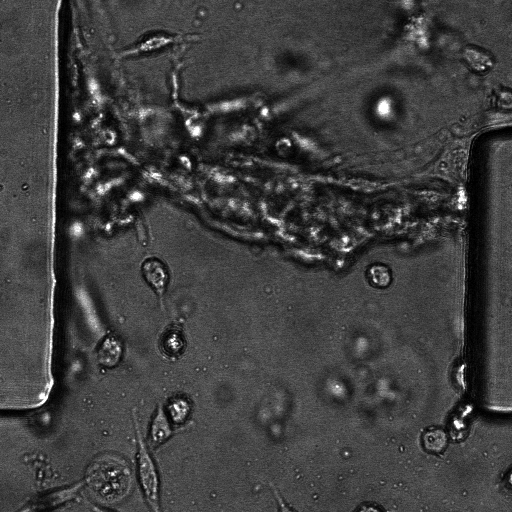
\includegraphics[width=1.0\textwidth]{211-digital_image_sample_bf-050714_s13_ch1_t85_z30}
\caption[sfs]{sdfsdf}
\label{fig:digital_image_sample_bf}
\end{figure}

\subsection{Edge detection}

%\begin{figure}[htbp!]
%\centering
%\includegraphics[width=1.0\textwidth]{}
%\caption[]{}
%\label{fig:canny_filter_bf}
%\end{figure}

\subsection{Blobs}

%\begin{figure}[htbp!]
%\centering
%\includegraphics[width=1.0\textwidth]{}
%\caption[]{}
%\label{fig:blob_detection_bf}
%\end{figure}

\subsection{Complex features and machine learning}

%\begin{figure}[htbp!]
%\centering
%\includegraphics[width=1.0\textwidth]{}
%\caption[]{}
%\label{fig:neural_nets}
%\end{figure}

%********************************** %Second Section  **************************************
\section{Basics of cell segmentation}

\subsection{Optical structure of the cell}

%\begin{figure}[htbp!]
%\centering
%\includegraphics[width=1.0\textwidth]{}
%\caption[]{}
%\label{fig:cell_structure}
%\end{figure}

\subsection{Cell shape}

%\begin{figure}[htbp!]
%\centering
%\includegraphics[width=1.0\textwidth]{}
%\caption[]{}
%\label{fig:cell_outlines}
%\end{figure}

\subsection{Fluorescence microscopy}

%\begin{figure}[htbp!]
%\centering
%\includegraphics[width=1.0\textwidth]{}
%\caption[]{}
%\label{fig:gfp_example}
%\end{figure}

%********************************** %Third Section  **************************************
\section{Review of studies on cell segmentation}

\subsection{Studies using GFP fluorescence data}

%\begin{figure}[htbp!]
%\centering
%\includegraphics[width=1.0\textwidth]{}
%\caption[]{}
%\label{fig:gfp_segmentation_example}
%\end{figure}

\subsection{Studies using brightfield data}

%\begin{figure}[htbp!]
%\centering
%\includegraphics[width=1.0\textwidth]{}
%\caption[]{}
%\label{fig:cp_segmentation}
%\end{figure}

\subsection{Review of studies}
